\documentclass[a4paper,12pt,twoside]{report}
\usepackage[left=2cm,right=2cm,top=2cm,bottom=3cm]{geometry}

\usepackage[utf8]{inputenc}
\usepackage{amsmath}
\usepackage[spanish, es-tabla]{babel}
\usepackage{amsfonts}
\usepackage{amssymb}
\usepackage{multirow, array} 
\usepackage{chngcntr}
\usepackage{graphicx}
\usepackage{subfig}
\usepackage{cite}
\usepackage{adjustbox}
\usepackage[table]{xcolor}
\usepackage{braket}

\usepackage{color}   %May be necessary if you want to color links
\usepackage{hyperref}
\hypersetup{
    colorlinks=true,
    linkcolor=black,
    urlcolor=magenta,
    citecolor=blue
}

\title{}
\begin{document}
\begin{center}
\thispagestyle{empty}
\fontsize{12pt}{12pt}\selectfont 

%%%%%%%%%%%%%%%%%%% PORTADA %%%%%%%%%%%%%%%%%%%%%%%%


\textbf {\huge Calibración del espectrografo EShel- II PF0011}
%\huge

\vspace{3cm}


{\large \textbf{Autor:}}

\vspace{0.5cm}

\large Jesús Alberto Sánchez Villafrades$^{1,2}$

\vspace{3cm}

{\large \textbf{Director}}\\

\vspace{0.5cm}

{\large Director: Luis Alberto Núñez$^{1,2}$}\\

\vspace{0.5cm}

{\large \textbf{Codirector}}\\

\vspace{0.5cm}

{\large Juan Pablo Uchima Tamayo $^{3}$}

\vspace{3cm}

\normalsize

\large Propuesta de trabajo de grado para optar al t\'itulo de F\'isico


\vspace{4cm}



\large $^1$Grupo de Investigaci\'on en Relatividad y Gravitaci\'on GIRG \\
\large  $^2$Grupo Halley de Astronom\'ia y Ciencias Aeroespaciales \\
\large  $^3$Universidad de la Serena \\
\large  Escuela de Física - 2020
  \end{center}
  
\newpage
%%%%%%%%%%%%%%%%%%%%%%FIN  DE LA PORTADA    %%%
%\leavevmode\thispagestyle{empty}\newpage

\newpage

%------------- Documento --------------
%%%%%%%%%%% PARA LA TESIS FINAL
\pagenumbering{roman}
\setcounter{page}{2}
%\input{Nota.tex}
%\input{Autorización}
%\addcontentsline{toc}{chapter}{Dedicatoria}
%\input{Dedicatoria.tex}
%\addcontentsline{toc}{chapter}{Agradecimientos}
%\input{Agradecimientos.tex}

%%%%%%%%%%%%%%%%%%%%%%%%%%%%%%%%%%%%%%%%%%%%%%%%%%%%%
\tableofcontents % indice de contenidos
\cleardoublepage
%\addcontentsline{toc}{chapter}{Lista de figuras}
\listoffigures % indice de figuras
%\addcontentsline{toc}{chapter}{Lista de tablas}
\listoftables % indice de tablas
%\addcontentsline{toc}{chapter}{Lista de símbolos}
%\input{Symbols/Symbols}
%\addcontentsline{toc}{chapter}{Resumen}
%\addcontentsline{toc}{chapter}{RESUMEN}
\newpage
\chapter*{RESUMEN}
\label{sec:resum}

\textbf{TÍTULO:} CARACTERIZACIÓN DE PERFILES ATMOSFÉRICOS PARA LA CADENA DE SIMULACIÓN DE LA COLABORACIÓN LAGO.\\

\textbf{AUTORA:} Jennifer Grisales Casadiegos.\\

\textbf{PALABRAS CLAVES: } Astropartículas, flujo de secundarios, atmósfera, simulaciones, cascadas aéreas extensas.\\

Uno de los objetivos del programa de clima espacial del \textit{Latin American Giant Observatory} (LAGO), es estudiar la influencia de la actividad solar en las variaciones del flujo de partículas secundarias, producidas durante la interacción de las astropartículas con la atmósfera. Con este fin, se realiza una cadena de simulaciones, que estima de forma detallada, el desarrollo del primario desde su ingreso a la atmósfera terrestre, hasta la respuesta en los detectores Cherenkov de agua. El presente trabajo, completa esta cadena de simulaciones, concentrándose en el estudio del efecto que tiene la atmósfera en el flujo de fondo de secundarios. Para ello, se desarrolló una metodología que permite la creación y uso de perfiles atmosféricos mensuales, para cualquier ubicación geográfica, en las simulaciones de EAS dentro del código CORSIKA. Además se demostró la pertinencia de reemplazar los modelos atmosféricos predeterminados por nuevos perfiles, basados Sistema Global de Asimilación de datos (GDAS), comprobando, que los nuevos modelos atmosféricos mensuales, son capaces de reproducir, en el flujo de secundarios, el efecto de los cambios de temperatura a lo largo del año, y permitiendo refinar las estimaciones realizadas.
%en el proceso de formación de cascadas aéreas extensas (EAS), más específicamente,
%\addcontentsline{toc}{chapter}{Abstract}
%\addcontentsline{toc}{chapter}{Abstract}
\newpage
\chapter*{ABSCTRACT}
\label{sec:abst}

\textbf{TITLE:} CARACTERIZATION OF ATMOSPHERIC PROFILES FOR THE LAGO SIMULATION CHAIN.\\

\textbf{AUTHOR:} Jennifer Grisales Casadiegos.\\

\textbf{KEYWORDS: } Astroparticle, particle flux, atmosphere, simulation, extensive air shower.\\

One of the main objectives of the Space Weather program of the Latin American Giant Observatory (LAGO), is to study the influence of the solar activity on the secondary particle flux  variations, produced during the interaction between astroparticles with atmosphere. To this end, a chain of simulations is carried out, which estimates in detail, the Primary's development, from its entry into the Earth's atmosphere, to the Water Cherenkov Detector response. This work, complete the simulation chain, focusing their interest in to study the atmospheric effect on the secondary particle flux. To do this it developed a metodology that allows the creation and use of monthly atmospheric profiles, for any localization, in the EAS simulations within the CORSIKA code. Futhermore, the relevance to using the new monthly profiles it was checked, becouse they are abble to reproduce in the secondary particle flux, the effect of the temperature changes along the year. This allows refine the estimates made.
%en el proceso de formación de cascadas aéreas extensas (EAS), más específicamente,

%%%%%%%%%%%%%%%%%%%%%%%%%%%%%%%%%%%%%%%%%%%%%%%%%%%%%Cambio de Numeración
\newpage
\pagenumbering{arabic}
\setcounter{page}{1}

\addcontentsline{toc}{chapter}{INTRODUCCIÓN}
\newpage
\chapter*{INTRODUCCIÓN}
\label{sec:intro}

Para el año 1912, el físico Victor Hess, mediante experimentos con globos aerostáticos y electrómetros, pudo evidenciar, que la ionización atmosférica aumenta proporcionalmente con la altitud. Había encontrado que el fondo de radiación presente, tenía un aporte significativo del espacio exterior, descubriendo así las astropartículas. Desde entonces, se han desarrollado decenas de experimentos alrededor del mundo, tanto en Tierra, como en el espacio, que intentan comprender a profundidad su origen, además de obtener información de fenómenos astrofísicos como explosiones de supernovas, kilonovas, entre otros. Adicionalmente, también se han desarrollado diversas aplicaciones en Tierra, que aprovechan la existencia de esta radiación por ejemplo, el detector Mu-Ray \cite{Mu-Ray}, el proyecto MuTe \cite{MuTe}, entre otros.\\

En esencia, el flujo de radiación medido en la superficie de la Tierra, es consecuencia principalmente, de partículas provenientes del espacio que llegan a la atmósfera e interactúan con ella. Este fenómeno está determinado por fenómenos físicos de dispersión, decaimientos y absorción. Además, para energías por debajo de $10^{15}$ eV, está modulado por el viento solar. La influencia de la actividad solar en el campo geomagnético y su relación con el funcionamiento de muchos dispositivos tecnológicos de la vida diaria, hacen que el transporte de partículas a través de la heliósfera sea un tema de gran interés en la física espacial. \\

Por tal razón, el \textit{Latin American Giant Observatory} (LAGO), ha desarrollado el programa de Clima Espacial, que busca entender la influencia del viento solar en el flujo de astropartículas, a partir de detectores de superficie. Dichos detectores pueden registrar partículas primarias de baja energía de forma indirecta, permitiendo obtener información de la actividad solar, complementando las observaciones que se realizan desde el espacio.\\

Con base en lo anterior, una de las tareas fundamentales  que se propone el programa de clima espacial de LAGO es estimar de forma precisa el flujo de partículas que llegan a nivel del suelo. Para tal fin, se ha desarrollado una secuencia de simulaciones, que tienen en cuenta el transporte de primarios en la heliosfera, el flujo de primarios a través de la magnetosfera, la llegada de primarios a la atmósfera, la formación de lluvias de secundarios o cascadas aéreas extensas (EAS), y la llegada de estos a los detectores de la colaboración.\\
%

En la actualidad, para el estudio de las EAS y su propagación a través de la atmósfera, LAGO hace uso de perfiles atmosféricos predefinidos en sofware CORSIKA. Para el caso de Bucaramanga, usa el perfil subtropical que corresponde a la región del globo en la que se ubica la ciudad. Sin embargo, se debe realizar un estudio más detallado que permita determinar la pertinencia de estos perfiles y la sensibilidad que tienen a variaciones en el flujo estimado.\\
%

Por lo anterior, el presente trabajo se concentra en el estudio del efecto que tiene la atmósfera en el flujo. Para esto, se ha desarrollado una metodología que permite la creación y uso de perfiles atmosféricos mensuales, para cualquier ubicación geográfica, dentro del código CORSIKA. En el capítulo 1, se realiza una breve revisión de los conceptos relacionados con las astropartículas y las cascadas aéreas extensas. Además, se describen algunos detalles relevantes de la estructura del código CORSIKA, tanto en los procesos de interacción como en las características de la atmósfera, y su modelado.\\

A continuación, en el capítulo 2, se presenta la forma como se estima el flujo de fondo de secundarios, y se introduce la metodología para crear perfiles atmosféricos mensuales, usando el Sistema Global de Asimilación de Datos (GDAS). En éste capítulo, se muestran los resultados de comparar el perfil atmosférico que actualmente se usa para la ciudad de Bucaramanga, contra los perfiles atmosféricos que fueron construidos para este trabajo.\\
%, evidenciando una diferencia significativa en los valores de densidad.\\

Finalmente, en el capítulo 3, se realiza un estudio detallado, de los efectos sobre el flujo de partículas, de las variaciones de densidad estimadas que fueron observadas mes a mes, y cómo estos efectos se relacionan con los cambios de temperatura, a lo largo del año. Además, se muestran las diferencias observadas en las estimaciones del flujo entre el perfil atmosférico subtropical, y los nuevos perfiles atmosféricos que fueron construidos. Esperándo con esto poder confirmar la importancia del uso de perfiles atmosféricos en cada sitio de la colaboración y completar la cadena de simulaciones de la colaboración LAGO.\\
%Estos resultados permitieron confirmar la importancia del uso de perfiles atmosféricos en cada sitio de la colaboración, y la metodología que se muestra en este trabajo, permite completar la cadena de simulaciones de la colaboración LAGO.\\

\newpage
\chapter{Marco teórico}
La espectroscopia estudia la interacción entre la radiación electromagnética y la materia,en astronomía esta radiación es emitida por estrellas y otros objetos celestes y al ser dispersada brinda mucha información de la fuente que la genero.\\
Para el caso del espectro visible esta Luz puede ser dispersada usando un prisma mediante el fenómeno de refracción o usando una rejilla de difracción, estos espectros dan información importante de las características físicas del objeto que las emite,están directamente relacionadas con la temperatura superficial del objeto así como con su composición química. Usando Efecto Doppler se puede tener información de la velocidad de rotación y traslación además de densidad y presión. \cite{utilidad}\\

\section {Principios de la espectroscopia.}
Todo elemento que  irradie luz presenta en esta luz información detallada de las propiedades constituyentes de dicho elemento así como su temperatura, esta luz esta compuesta de múltiples longitudes de onda que son separadas y se pueden observar en un sensor ccd en forma de linea espectral, que es la distribución de  la intensidad en función de la longitud de onda o la frecuencia  de luz dispersada.

\subsection {Espectros y lineas espectrales.}

Históricamente las lineas espectrales fueron llamadas así ya que se  presenta como lineas de obscuridad o luminosidad en la salida de un espectroscopio luego de la dispersión, por esto la forma de las lineas dependen del instrumento que se este utilizando.\\
Estas lineas son de origen cuántico y se generan por la transición de 2 niveles de energía, estos puede dividirse en 3 tipos,las lineas espectrales continuas ,de emisión y las de absorción.\cite{troccoli}


\textbf{Espectro Continuo:}
Se define un espectro continuo cuando la franja de colores  pasa de un color a otro sin ninguna interrupción de franjas negras entra color y color como se presente en la figura 1, se puede observar esto con la luz blanca y en general cualquier solido o gas sometido a altas presiones o temperaturas presente un espectro continuo.


\begin{figure}[htb!]
\centering

\includegraphics[width=0.7\textwidth]{images/1.png}
\caption[Espectro continuo.]{Espectro continuo.\cite{libro}}
 \label{fig2}
\end{figure}

\textbf{Espectro de emisión :} Un gas a baja presión y excitado a altas temperaturas produce un espectro de emisión,estos espectros constan de rayas de diversos colores separadas por amplias zonas  negras en las que no se observa luz ver figura 2. Este tipo de espectro se da cuando los electrones en los átomos de estos gases excitados absorben energía de la fuente que los esta excitando  y saltan a orbitas superiores , la emisión tiene lugar cuando los electrones caen a niveles mas bajos emitiendo este exceso de energía en forma de fotones con una frecuencia característica propia de cada elemento.


 \begin{figure}[htb!]
\centering
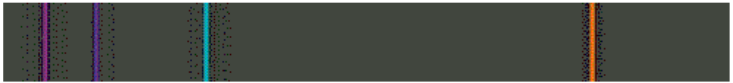
\includegraphics[width=0.7\textwidth]{images/2.png}
\caption[Descripción versión comprimida]{El espectro de emisión del hidrógeno \cite{articulo1}}
 \label{fig3}
\end{figure}


\textbf{Espectro de absorción :} Este tipo de espectro se da cuando se hace pasar luz blanca a través de un gas frío a baja presión, el espectro que se observa presenta un fondo de color con franjas negras, con la característica principal de que las lineas de absorción aparecen en el mismo lugar que las lineas de emisión.\\
En astronomía las fuente luminosa generalmente es una estrella, la luz proveniente de la estrella atraviesa capas de gas propia de la atmósfera, las lineas de absorción dependerán estrictamente de la composición química del gas, esta absolverá fotones de una u otra longitud de onda dejando las franjas obscuras características de espectro de absorción.


\begin{figure}[htb!]
\centering
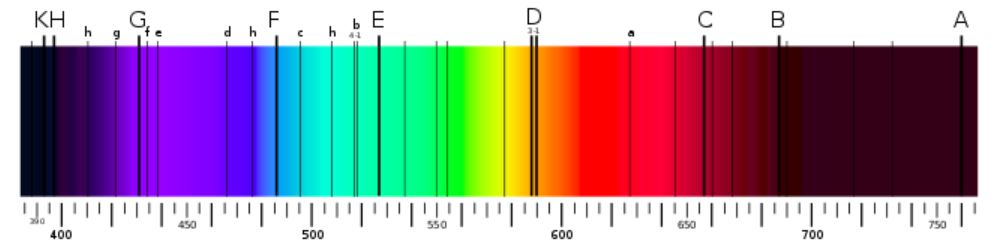
\includegraphics[width=0.7\textwidth]{images/3.png}
\caption[Descripción versión comprimida]{Espectro solar en el que se aprecian las líneas principales de von Fraunhofer. \cite{articulo1}}
 \label{fig4}
\end{figure}

%falta citar de https://culturacientifica.com/2019/08/13/los-espectros-de-absorcion-de-los-gases/

Los anteriores espectros tienen su explicación en las leyes de kirchof  que se presentan a continuación.

-Un espectro continuo se produce por un un solido incandescente o un gas a alta presión.

-Un espectro de emisión se produce por un gas incandescente a baja presión.

- Cuando se hace pasar luz blanca a través de un gas a baja presión y baja temperatura se produce un espectro de emisión.

\subsection {Radiación de cuerpo negro}
Es bien conocido el fenómeno por el cual todos los cuerpos que se encuentran por encima del cero absoluto presentan radiación electromagnética, a altas temperaturas se habla de incandescencia pues las longitudes de onda de emisión se encuentran en el espectro visible (entre 400 y 700 nm) aun a bajas temperaturas  el objeto seguirá irradiando pero ahora en el infrarroja (longitudes de onda superiores a 700 nm).\cite{libro2} \\
Kirchoff propuso en 1860   una hipótesis  de radiación para los cuerpo en equilibrio , la denomino radiación de cuerpo negro, esta muestra como la radiación tiene un patrón regular que depende de la temperatura.Mas tarde  Wein y Plank  hicieron el desarrollo matemático e este fenómeno, que se puede modelar como:


\begin{equation}
    \lambda_{max}=\frac{0.002898}{T}
\end{equation}


Donde $ \lambda$ es la longitud de onda máxima emitida por el cuerpo y T es la temperatura en grados Kelvin.\\

\textbf{Ley de desplazamiento de Wien:}Durante el año 1893 Wien basándose en argumentos estadístico dedujo que la distribución normal de radiación, como era conocida hasta la fecha se modelaba  con la expresión:  


\begin{equation}
    I(\nu,T)=\nu^3 f \left(\frac{\nu}{T}\right)
\end{equation}


Donde $f\left(\frac{\nu}{T}\right)$ es desconocida pero solo puede depender de $\nu$ y de T.\\
Sin embargo Wien usando los datos de los experimentos realizados en la época pudo llegar a una expresión mas detallada para la ecuación  (2).  


\begin{equation}
    I(\nu,T)= a \nu^{3} e^{-b(\frac{\nu}{T})}
\end{equation}{}


Donde a y b son constantes que se determinan durante el experimento.\\
Esta expresión modelaba muy bien los experimentos  reproducidos en la época y daba una explicación satisfactoria a los resultados empíricos que demostraban que la frecuencia de radiación mas intensa emitida por un cuerpo negro $\nu_{max}$ aumenta linealmente con la temperatura.

\begin{figure}[htb!]
\centering
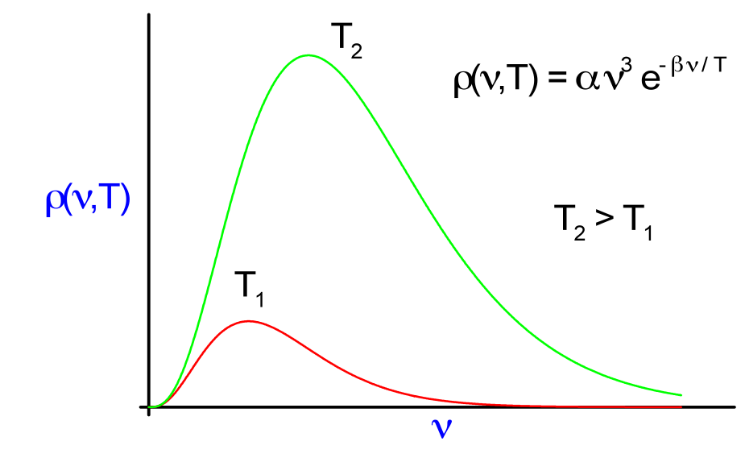
\includegraphics[width=0.6\textwidth]{images/5.png}
\caption[Descripción versión comprimida]{Wien propuso la expresión para la distribución normal de radiación que predice el pico de la distribución de corriente lineal con la la temperatura T.\cite{plank}}
 \label{fig1}
\end{figure}

\textbf{La deducción de Planck:}Para el año 1900 Otto Lummer y Ernst Pringsheim junto con otros 2 investigadores Heinrich Rubens y Ferdinand Kurlbarm realizaron múltiples experimentos y notaron que la ecuación de Wien (1.3) no concordaba con los experimentos a frecuencias bajas, a estas frecuencias la distribución normal de radiación notaron que eran directamente proporcional al cuadrado de la frecuencia por la temperatura.

\begin{equation}
    I(\nu,T) \sim \nu^{2} T
\end{equation}{}






%http://www.quimicafisica.com/radiacion-cuerpo-negro-hipotesis-planck.html





\subsection {Diagramas de Hertzsprung-Russell}


La espectroscopia permitió la construcción del diagrama Hertzsprung-Russell, el cual se desarrollo inicialmente en la Universidad de Harvard.
Este diagrama muestra la etapa de evolución de las estrellas con las líneas espectrales que señala el estado de los elementos químicos presentes en ellas. La figura 2.3 muestra como se relacionan las estrellas en tamaño, color, luminosidad, clase espectral y la magnitud absoluta. Cada punto en este diagrama representa una estrella en el firmamento, cuya magnitud y clase espectral absoluta han sido determinadas. Los datos se agrupan en: estrellas de secuencia principal, supergigantes, gigantes y enanas
blancas.


%\subsection {Lineas de franhofer}



\newpage
\chapter{Objetivos}

%%%%%%%%%%%%%%%%%%%%%%%%%%%%%%%%%%%%%%%%%%%%%%%%%%%%%%%%%%%%%%%%%%%%%%%%%%%%%%%%%%%%%%%%%%%%%

\begin{itemize}
\item \textbf{Objetivo General}

Realizar el montaje, calibración y puesta en funcionamiento de ESPECTRÓGRAFO eShel II con el que cuenta el Grupo Halley de Astronomía y Ciencias Aeroespaciales de la Universidad Industrial de Santander.\\

\item \textbf{Objetivos Específicos}
\end{itemize}

\begin{itemize}


\item Verificar el enfoque del lente colimador del espectrógrafo eShel II verificándolos con lineas de lamparas de emisión.

\item Realizar la calibración pixel-Longitud de onda mediante el software IRAF, usando lamparas de calibración con espectros conocidos.

\item Realizar los cálculos de la masa de aire para la ciudad de Bucaramanga de forma teórica.

\end{itemize}
\newpage


\newpage
\chapter{Metodolog\'ia}

El telescopio CDK 17 (corrected Dall-kirkham) es un telescopio de tubo ópticoo de diseño abierto, hecho en fibra de carbono con un paso de 43 kg, cuenta con 2 lentes de 90 mm (aplanadores de campo) y 2 espejos. 
Un espejo primario elipsoidal con una apertura de 432 mm y una relación focal de f/2,6 y un espejo secundario con una apertura de 159 mm con forma esférica.\\
Posee un enfocador Hedrik 3.5 y tres ventiladores en la parte inferior y 4 en las laterales del tubo óptico, todo esto acoplado a una montura ecuatorial Paramount ME II.\\
La montura Paramout ME II tiene un eje de contrapeso DEC 47 CM  de largo y 48 mm de diametro, 2 contrapesos de 14 Kg, un rodamiento de declinacion de 48 puntos de contacto, con una capacidad de carga de 140 Kg.


Para cumplir con los objetivos planteados se llevara la siguiente metodología.

\begin{itemize}

\item[1] Montaje del espectrógrafo con sus respectivo modulo de calibración y acople al telescopio.

\item[2] hacer el calculo de forma experimental de la rendija del espejo que permite el paso de luz al espectrógrafo.

\item[3] Realizar la captura de imágenes limpias de diferentes lamparas de emisión de laboratorio con el fin de garantizar que los elementos dispersores del espectrógrafo estén alineados con la cámara y se puedan reproducir espectros conocidos.

\item[3] Se calibrara la Montura robotizada PARAMOUNT  usando el software T-Point para garantizar un correcto apunte del telescopio al objeto de interés.



 
\end{itemize}

%%%%%%%%%%%%%%%%%%%%%%%%%%%%%%%%%%%%%%%%%%%%%%%%%%%%%%%%%%%%%%%%%%%%%%%%%%%%%%%%%%%%%%%%%%%%%%


%%%%%%%%%%%%%%%%%%%%%%%%%%%%%%%%%%%%%%%%%%%%%%%%%%%%%%%%%%%%%%%%%%%%%%%%%%%%%%%%%%%%%%%%%%%%%%
\section{Cronograma de Actividades}	
%%%%%%%%%%%%%%%%%%%%%%%%%%%%%%%%%%%%%%%%%%%%%%%%%%%%%%%%%%%%%%%%%%%%%%%%%%%%%%%%%%%%%%%%%%%%%%


\begin{center}
{\small
\begin{tabular}{|c|c|c|c|c|c|c|c|}
\hline

\textbf{Mes}/\textbf{Actividad}&\textbf{Act 1.1}&\textbf{Act 1.2}
&\textbf{Act 1.3}&\textbf{Act 2}&\textbf{Act 3}&\textbf{Act 4}&\textbf{Act 5}\\

\hline

Enero&$\bigotimes$&&&&&&\\

\hline

Febrero&$\bigotimes$&$\bigotimes$&&&&&\\

\hline

Marzo&&$\bigotimes$&$\bigotimes$&&&&\\

\hline

Abril&&&$\bigotimes$&&&&\\

\hline

Mayo&&&$\bigotimes$&$\bigotimes$&&&\\

\hline

Junio&&&$\bigotimes$&$\bigotimes$&&&\\

\hline
Julio&&&$\bigotimes$&$\bigotimes$&$\bigotimes$&&$\bigotimes$\\

\hline

Agosto&&&&&$\bigotimes$&$\bigotimes$&\\

\hline 

Septiembre&&&&&&&$\bigotimes$\\

\hline
Octubre&&&&&&&$\bigotimes$\\
\hline

\end{tabular}
}
\end{center}
\newpage
\chapter{CONCLUSIONES}


Se construyó una metodología que permite crear perfiles atmosféricos promediados mes a mes, para cualquier ubicación geográfica, usando el código GDASTOOL. Esta metodología propone la extracción de datos de dos horas del día diferentes: 0:00 y las 12:00 UTC-5, para todos los días del año. Se crearon perfiles atmosféricos para la ciudad de Bucaramanga (7.11 N, 73.11 E) y se construyeron 12 perfiles para cada mes del año 2018, que se contrastaron con el perfil atmosférico Subtropical que viene predeterminado en CORSIKA. Este trabajo, completa la secuencia de simulaciones que LAGO estableció en el programa de clima espacial, el cual busca estudiar los fenómenos relacionados a la  modulación que realiza el viento solar al flujo de secundarios que se pueden detectar en tierra.\\

Adicionalmente, se realizó una validación, construyendo perfiles atmosféricos para el Observatorio Pierre Auger, y contrastándolos con el perfil basado en GDAS que actualmente usa el Observatorio. Las simulaciones arrojaron que el modelo reconstruido reproduce el resultado de las atmósferas mensuales estándar de Malarg\"ue construidas con GDAS, con una diferencia porcentual por debajo del 20$\%$ después de los 400 $g/cm^{2}$. Además el comportamiento de la EAS que se obtiene con la atmósfera reconstruida muestra una diferencia de $\approx$ 2$\%$ en el valor del $X{max}$.\\

Con estos perfiles construidos, se contrastó la diferencia de  densidad atmosférica, en relación al perfil subtropical predeterminado en CORSIKA, y se observaron diferencias que llegan hasta el 58$\%$, en los primeros 30 km como se mostró en la figura \ref{fig:fig16}.\\
%Se observa una diferencia notable que se incrementa rápidamente en los primeros 4 km hasta llegar a los 250 $g/cm^{2}$. Esto corresponde a un 58$\%$ de diferencia. Luego esta diferencia  disminuye, pero se mantiene por encima del 40$\%$.

Así mismo, se estudió el efecto de estos perfiles atmosféricos en el flujo de fondo de secundarios sobre Bucaramanga y se confirmó la relación que tienen estos perfiles con la variación de temperatura mensual a lo largo del año. Se evidenció una diferencia en el flujo total entre 10,22$\%$ y el 24,12$\%$ correspondientes a los meses de noviembre y abril respectivamente. De forma similar, para los muones estas diferencias están entre 9,58$\%$ y 22,25$\%$. Este resultado permite confirmar que las variaciones atmosféricas a lo largo del año, pueden ser evidenciadas en el flujo de secundarios a nivel del suelo.\\

%una diferencia significativa, entre los perfiles mensuales y el subtropical. Es constante en el transcurso del año, permitiendo concluir que este perfil predeterminado por CORSIKA no es el perfil adecuado para la ciudad, puesto que sobrestima el flujo significativamente.\\
%%se obtiene una diferencia en el flujo total entre 10,22$\%$ y el 24,12$\%$ correspondientes a los meses de noviembre y abril respectivamente. De forma similar, para los muones estas diferencias están entre 9,58$\%$ y 22,25$\%$. Este resultado responde finalmente a la interrogante planteada en el capítulo anterior. Además, permite concluir que las variaciones atmosféricas a lo largo del año, pueden ser evidenciadas en el flujo de secundarios a nivel del suelo, incluso en regiones tropicales como Bucaramanga.\\
También, se estudió el efecto de los perfiles atmosféricos en el desarrollo de las EAS generadas por partículas individuales. Se encontró que el perfil atmosférico cambia levemente la distribución longitudinal de secundarios, observando un mayor número de partículas cerca al $X_{max}$. Sin embargo, las diferencias en la posición del $X_{max}$ no superan el 8$\%$.\\

Finalmente, cabe resaltar que la metodología presentada, puede ser usada en cualquier ubicación geográfica, donde se requieran perfiles atmosféricos en base a GDAS, que recojan información suficiente y estable de las variables atmosféricas, en periodos determinados de tiempo. Los códigos que permiten extraer y crear los perfiles atmosféricos mensuales están disponibles de forma libre, en el repositorio web: \url{https://github.com/jennifergc/Tesis_Pregrado}. \\

%Esta cadena de simulaciones se establece en tres bloques principales: el cálculo de los efectos del campo geomagnético en la propagación de partículas cargadas, que contribuyen a la radiación de fondo a nivel del suelo y que se caracterizan por la rigidez de corte en cada sitio LAGO \footcite{lagoSW}. La estimación del flujo de partículas secundarias al nivel de los detectores, originado por la interacción de los primarios con la atmósfera, parte en la que se concentra este trabajo. Y, la obtención de la respuesta del detector para los diferentes tipos de  partículas secundarias \footcite{andrei}.

Los resultados de este trabajo de grado, han sido presentados en  el VI Congreso Colombiano de Astronomía y Astrofísica CoCoA, celebrado en la ciudad de Medellín, con la ponencia: \textit{Estimación del flujo de astropartículas usando el Sistema Global de Asimilación de Datos, para la colaboración LAGO}, y en el 11th Workshop of the Latin American Giant Observatory LAGO, celebrado en la ciudad de Buenos Aires, con la ponencia: \textit{Generación de perfiles atmosféricos con GDAS para LAGO}.


%\input{chapters/APENDICE_A.tex}
%\input{chapters/APENDICE_B.tex}
%\input{chapters/APENDICE_C.tex}


\newpage
%%%%%%%%%%%%%%%%%%%%%%%%% Bibliografia %%%%%%%%%%%%%%%%%%%%%5
\cleardoublepage
\addcontentsline{toc}{chapter}{Bibliografía}%para que aparezca en la tabla de contenidos
\bibliographystyle{unsrt}
\bibliography{Bibliography/Tesis.bib}
%Archivo con las referencias bibliográficas, creado en JabRef (o manualmente)

\end{document}
